\subsection{Semiconducting Quantum Dots}

Due to their practical application and rather easy, yet not really repeatable fabrication semiconductor quantum dots have made a vast impact in all technology. Their potential confinement in all three directions allows to profit from many new possibilities, not known in solid state physics before.
We can easily distinguish three different categories for their production which are:
\begin{itemize}
\item Self assembled QDs
\item Colloidal QDs
\item Electrostatically definded QDs 
\end{itemize}
Considering the fact that we are only using the second ones, we will mainly focus on them. 

\subsubsection{Colloidal Quantum Dots}
To put it straightforward, CQDs are semiconductor crystal of nanometre scale size, with diameter less than twice the Bohr radius, which are synthesized(deployed) by nucleation in colloidal solutions. They are surrounded and restricted by surfactant molecules called ligands. 

\begin{figure}[H]
\centering
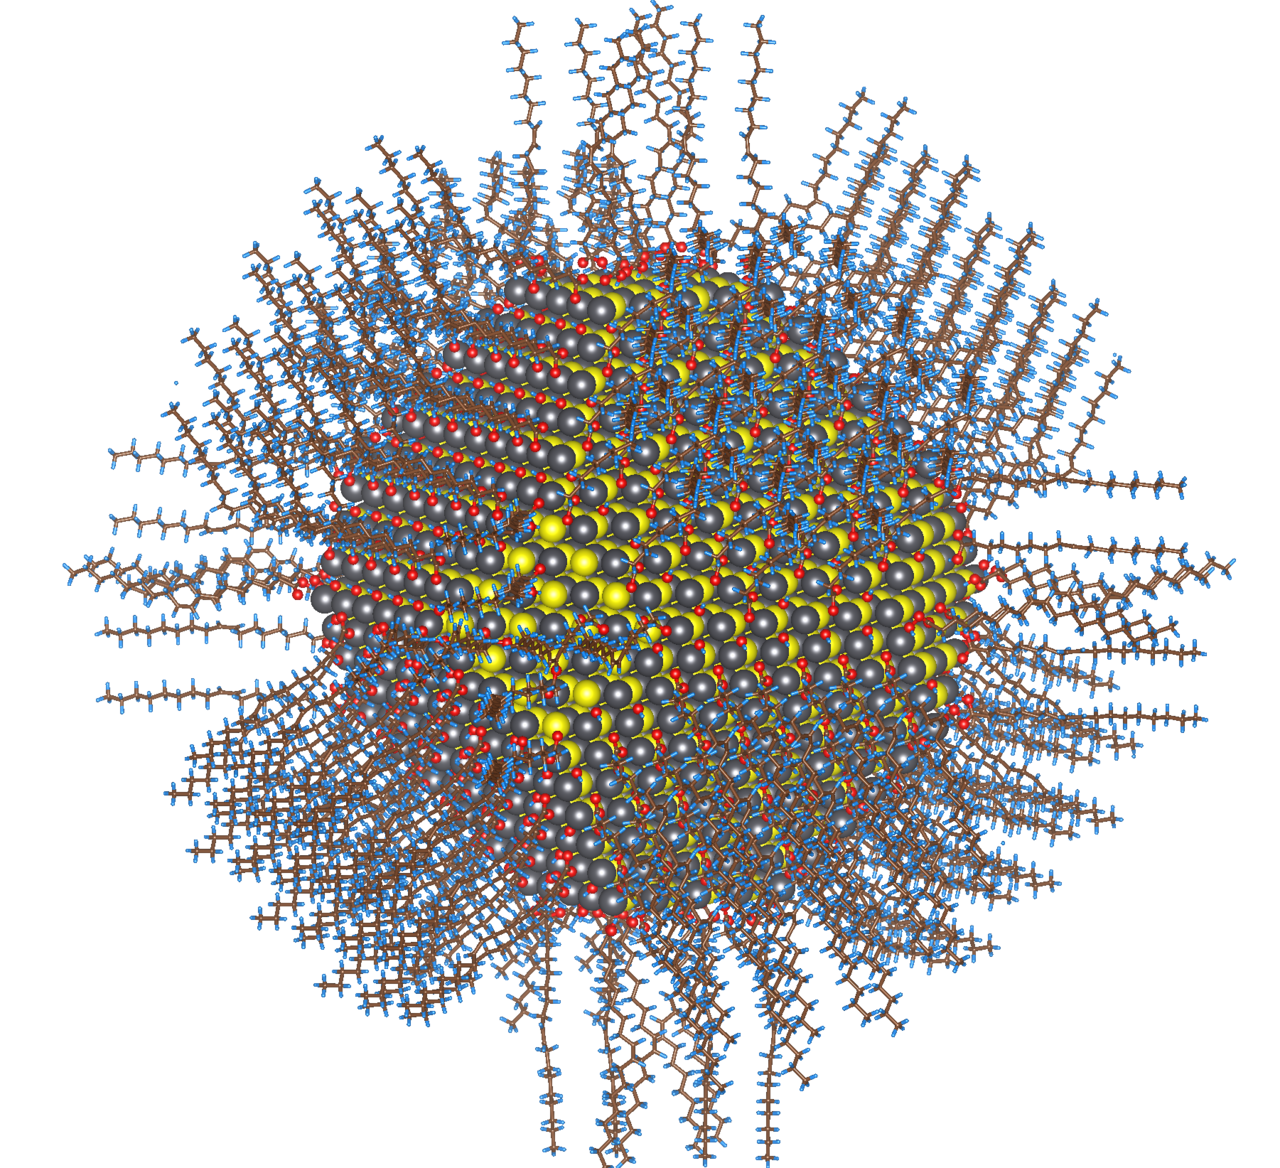
\includegraphics[width=0.4\textwidth]{ch2/colQD}

\caption{Image of ideal CQD composed of selenide with passivation with oleic acid, oleyl amine and hydroxyl ligands (\url{https://www.wikiwand.com/en/Quantum_dot})}
\end{figure}

\noindent They have manifested to provide a development of numerous types of optoelectronic devices including photo-diodes and PV devices. The properties of CQDs are easily adjusted by changing the volumetric features of nano-particles similarly to metallic nano-particles in plasmonic transport. \cite{Abdelhady2015} \cite{G.D.Scholes2003}

\noindent Even though we don't focus on the synthesis of particular used CQDs, it is instructional and scientifically appropriate to be slightly familiar with it. It consists of three-component solutions, which are precursors, organic surfactants and solvents. In order for get the precursors transformed into single chains called monomers, the probe is heated to high temperature(they have enough energy to get separated), then, when there's enough of them, the monomers are growing into crystals. Of course, the temperature shall be manipulated with a dose of care because when it's too high the crystals aren't forming fine or at all. When we achieve optimal saturation of monomers, we get quite even growth of all particles, (small ones grow faster than the heavy ones) and it has to be sustained in order for the homogeneity to be achieved.
Typically, CQDs create alloys, binary or ternary, and contain 100 to $10^5$ atoms. Usually, they confine all carriers inside the volume.
\subsubsection{Quantum dot size}
With changing the size of the nano-particle we can control the band gap over significant range of spectrum. Yet, practically, the width of the nano-particle is estimated from the energy band gap.
 \cite{Yu2003}
 
\subsubsection{Quantum dot shape}
The geometry in physics plays an important role, there is no question about that. It is obviously not different for Quantum Dots. The quantum confinement strongly depends on the shape and dimensional geometry. The ability to control the growth of certain form allows the nano-particles to exhibit a variety of properties. 

\subsection{Core-shell CQDs}     
Modification of the standard synthesis methods allows us to create new behaviour and improvements in nano-structures characteristics. For example, in this method, same type, but different semiconducting nano-crystals are grown around the first ones(core). They tend to achieve better luminescence than the former because we simply drastically cut the possibility of non-radiative recombinations between energy levels. We can differ type 1 structures using conduction band of the core below the shell energy level(the core confines all carriers inside because of the energy minimisation) and in the second type, the energy levels are mixed so only one type of carriers is confined to the shell and the core. \cite{phdsemi}

\begin{figure}[h]
\centering
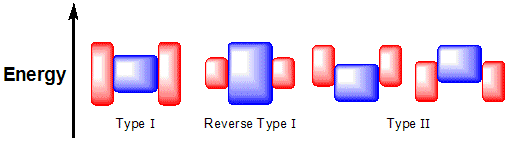
\includegraphics[width=\textwidth]{ch2/Core_shell_types}
\caption{Types of Core-Shell CQDs(red color is core energy structure), we can see that in the first type both electrons(smallest energy) and holes(biggest energy) are confined beneath the core. (\url{https://commons.wikimedia.org/wiki/File:Core-shell_types.png})}
\end{figure}

\subsection{CQD super-crystal}
With CQDs we can even create super-lattices(layers of few materials which create a periodic structure). In order to achieve the fine quality of them we need to have an absolutely outstanding transport properties. \cite{tranSupLat}
\subsubsection{Further reading}
More about synthesis and theory of nano-crystals and thermodynamics can be read in \cite{Klimov}, \cite{crystal}